%************************************************
\chapter{Implementation}\label{ch:implementation}
%************************************************

This chapter introduces a prototype implementation of the design that was presented in chapter~\ref{ch:design}. As is the nature of a prototype, not all features are implemented, and the following section will outline the objectives and scope of the prototype before going into implementation details.

\section{Goal and Scope}

The objective of the prototype is to showcase that the proposed protocol can be used to support the proposed design. In particular we partially implement scenarios ``Registration with a Service Provider'' (table~\ref{sc:register}) and ``Establishing a session'' (table~\ref{sc:auth}). 

These scenarios will be implemented to first of all to demonstrate, that the proposed authentication protocol for registration and authentication can be implemented and executed, exactly as described in chapter~\ref{ch:protocol}, using the specified cryptographic primitives.

Second, we want to show that the protocol can also be implemented in a distributed fashion, across four different hardware platforms: smartwatch, smartphone, browser-client and server, where each party executes their part of the protocol correctly. Herein also lies the challenge of getting the devices to communicate with low latency and stably in a manner that supports continuous authentication.

Third, we want to show that a proximity-based authentication mechanism is feasible to implement, and that a continuous authentication session can be established and will be interrupted whenever the watch and phone is not in proximity of the client.

Lastly, we want to include user awareness and explicit consent in our prototype, in order to demonstrate that some of the more usability related properties of our scheme, is also possible to implement in practice.

All other features, such as ``Unlocking the Authenticator'' (table~\ref{sc:unlocking}), and thereby also monitoring if the user is wearing the \gls{authenticator}, and ``Theft and Lost'' (table~\ref{sc:theft}), are left out of scope.


\begin{comment}
We have implemented a prototype system that serves to demonstrate that our envisioned scheme and protocol, is actually possible to implement and use in practice. We want to make it clear from the beginning, that the system is a prototype, and therefore doesn't include all of the envisioned functionality as proposed in chapter~\ref{ch:design}, but only a subset of the functionality which we consider most essential. 
The most significant goal of the prototype is, first of all, to demonstrate that the proposed authentication protocol for registration and authentication can be implemented and executed exactly as described in chapter~\ref{ch:protocol} using the specified cryptographic primitives. Second, we want to show that the protocol can also be implemented in a distributed fashion, across four different hardware platforms: smartwatch, smartphone, browser-client and server, where each party executes their part of the protocol correctly. Herein also lies the challenge of getting the devices to communicate with low latency and stably in a manner that supports continuous authentication. Third, we want to show that a proximity-based authentication mechanism is feasible to implement, and that a continuous authentication session can be established and will be interrupted whenever the watch and phone is not in proximity of the client. Lastly, we want to include user awareness and explicit consent in our prototype, in order to demonstrate that some of the more usability related properties of our scheme, is also possible to implement in practice.
All of the functionality mentioned above we are able to demonstrate with the current state of our implementation, however some functionality of the proposed scheme is not included in the implementation. Below is a short list of functionality that is excluded in our implementation but is part of design(chapter~\ref{ch:design}). The list only represents the most significant functionality that is excluded in our prototype and may therefore be incomplete. 
The implementation does not include:
\begin{itemize}
    \item The ability to verify ownership of the smartwatch (anyone in possession of watch and phone can authenticate).
    \item The ability to monitor that the user is actively wearing the watch. (the watch can be held in a pocket, or lay on a table and still authenticate).
    \item Configuration of when to use explicit consent and awareness (always uses both explicit consent and awareness).
    \item The `lockdown' feature. (no way to 
    \item Multiple instances of participating parties (only implemented and tested with one \gls{sibling}, one \gls{authenticator}, one \gls{client} and one \gls{server}).
\end{itemize}
\end{comment}

\section{Solution Description}
The implemented prototype system is based on the scheme design described in chapter \ref{ch:design} and consists of the 4 main components:
a smartphone acting as \gls{authenticator}, a smartwatch acting as \gls{sibling}, a browser acting as \gls{client} and a server application acting as \gls{server}.

The attentive reader might notice that the roles of the smartwatch and smartphone are switched in the prototype compared to the original design. We experienced stability issues when the watch was the party communicating with the client, and for ease of implementing the prototype, the roles are therefore reversed.

%we have implemented it such that the \gls{client} communicates with the smartphone and not the smartwatch. The watch only communicates with the phone. Therefore in accordance with the protocol specification and the specified sequence, that messages are supposed to be sent in, we have that the phone is \gls{authenticator} and the watch is \gls{sibling}.

The \gls{authenticator} and \gls{sibling} are implemented as background services that run on a user's smartphone and smartwatch respectively. The main responsibilities of the \gls{authenticator} and \gls{sibling} are to generate keys, decrypt challenges, and exchange messages that allow for user registration and continuous authentication. The implementation follows the specified protocol (chapter~\ref{ch:protocol}), in terms of when and where different cryptographic computations are carried out, and the sequence in which messages are exchanged between the 4 parties for registration and authentication.
Both \gls{authenticator} and \gls{sibling} notifies the user whenever authentication or registration processes are successful. Additionally the \gls{authenticator} (smartphone) also prompts the user to actively accept or decline incoming registration requests from the \gls{client}. The notifications that requires explicit consent from the user is shown in figure~\ref{fig:watch} and \ref{fig:phone}.



\begin{figure}[bth]
        \myfloatalign
        \subfloat[Passive notification]
        {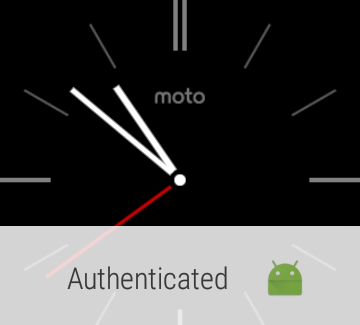
\includegraphics[width=.45\linewidth]{gfx/notification_auth_bar}} \quad
        \subfloat[When selected]
        {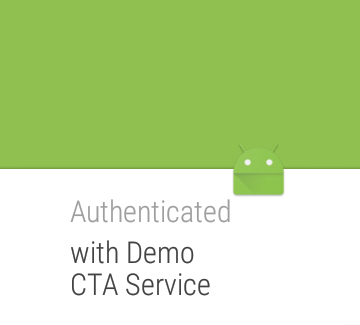
\includegraphics[width=.45\linewidth]{gfx/notification_auth}} 
        \caption{Example of notifications on the watch}
        \label{fig:watch}
\end{figure}

\begin{figure}[bth]
        \myfloatalign
        \subfloat[Registration notification]
        {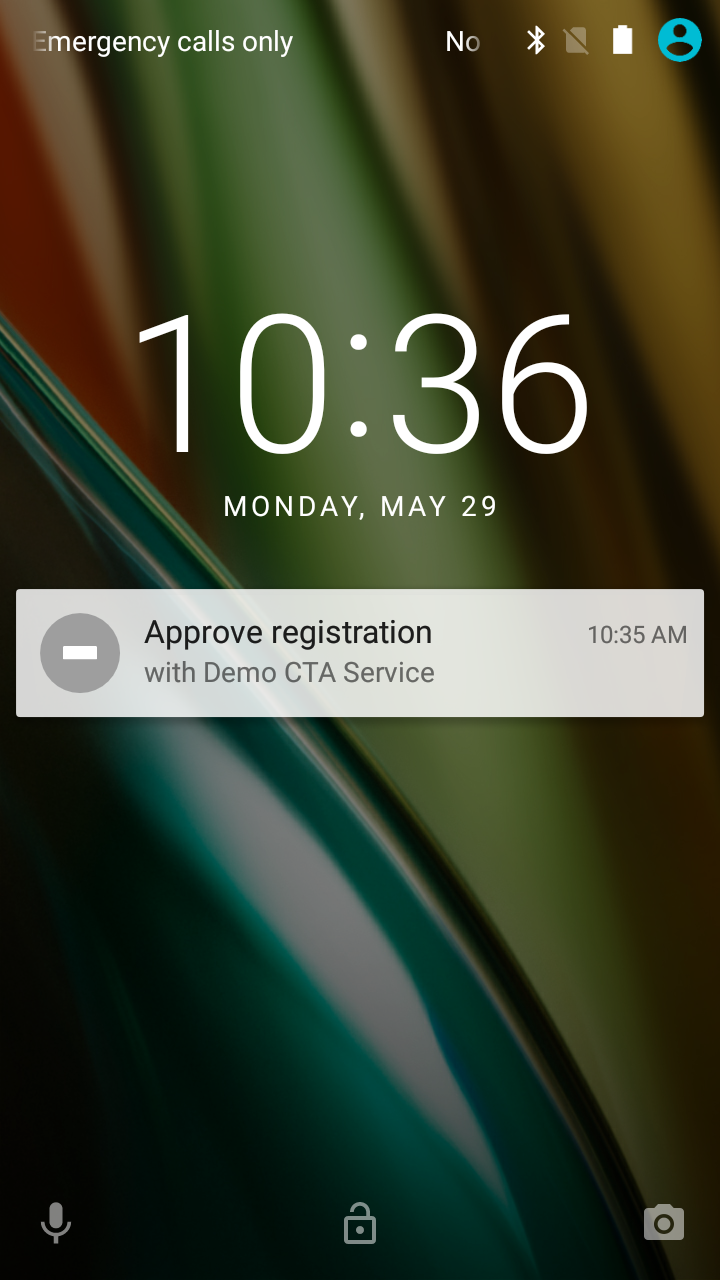
\includegraphics[width=.45\linewidth]{gfx/notification_register_phone}} \quad
        \subfloat[When selected]
        {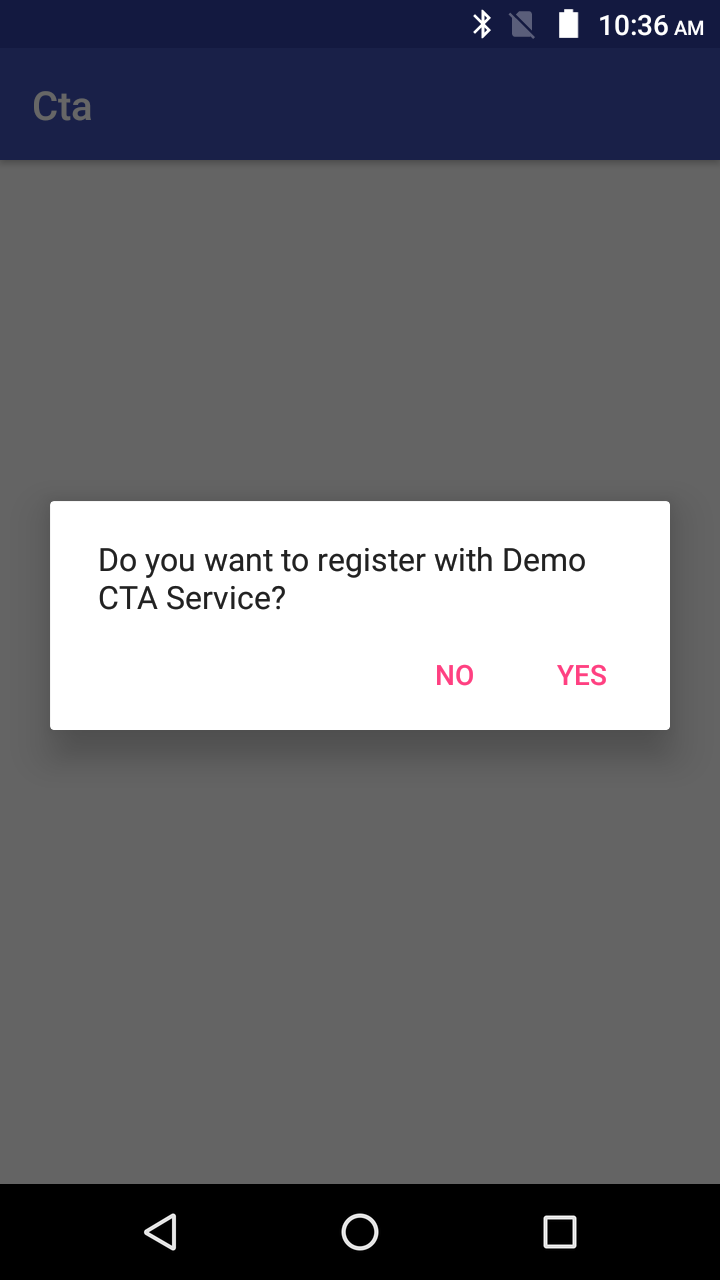
\includegraphics[width=.45\linewidth]{gfx/notification_register_approve}} 
        \caption{Example of explicit consent on the phone}
        \label{fig:phone}
\end{figure}

The \gls{server} is implemented as a server application that receives requests from the \gls{client}. Upon registration requests from the \gls{client}, the server is responsible for checking that the supplied username is available, and not already in use. If available it will respond to the \gls{client}, which will then initiate the registration process as specified in the protocol. Upon authentication requests from the \gls{client}, the server is responsible for encrypting new challenge ciphers and waiting for the \gls{client} to respond back with the correct cleartext message. Upon successful authentication the server generates a new token with a set expiration time, that is returned to the \gls{client}. This token allows the \gls{client} to authenticate with the \gls{server} as long as it is valid.

The \gls{client} is implemented as a small web application that runs in a browser. The \gls{client} is responsible for receiving input from the user, in the form of instructions of when to authenticate and register the user. Before either authentication or registration can be started from the \gls{client}, it must establish a connection with an \gls{authenticator} and a \gls{server} so that it can exchange protocol messages between the two parties. The client provides a simple user interface with a `pair' button used to select the correct \gls{authenticator} from a list of nearby Bluetooth devices. It has a field for typing a username, a button to perform registration and one to perform authentication. It also shows a log for displaying output from the client itself and response messages from its communicating parties. Lastly, it has a button used to interrupt the continuous authentication cycle with the \gls{server}, available whenever the client is authenticated.

\begin{figure}
       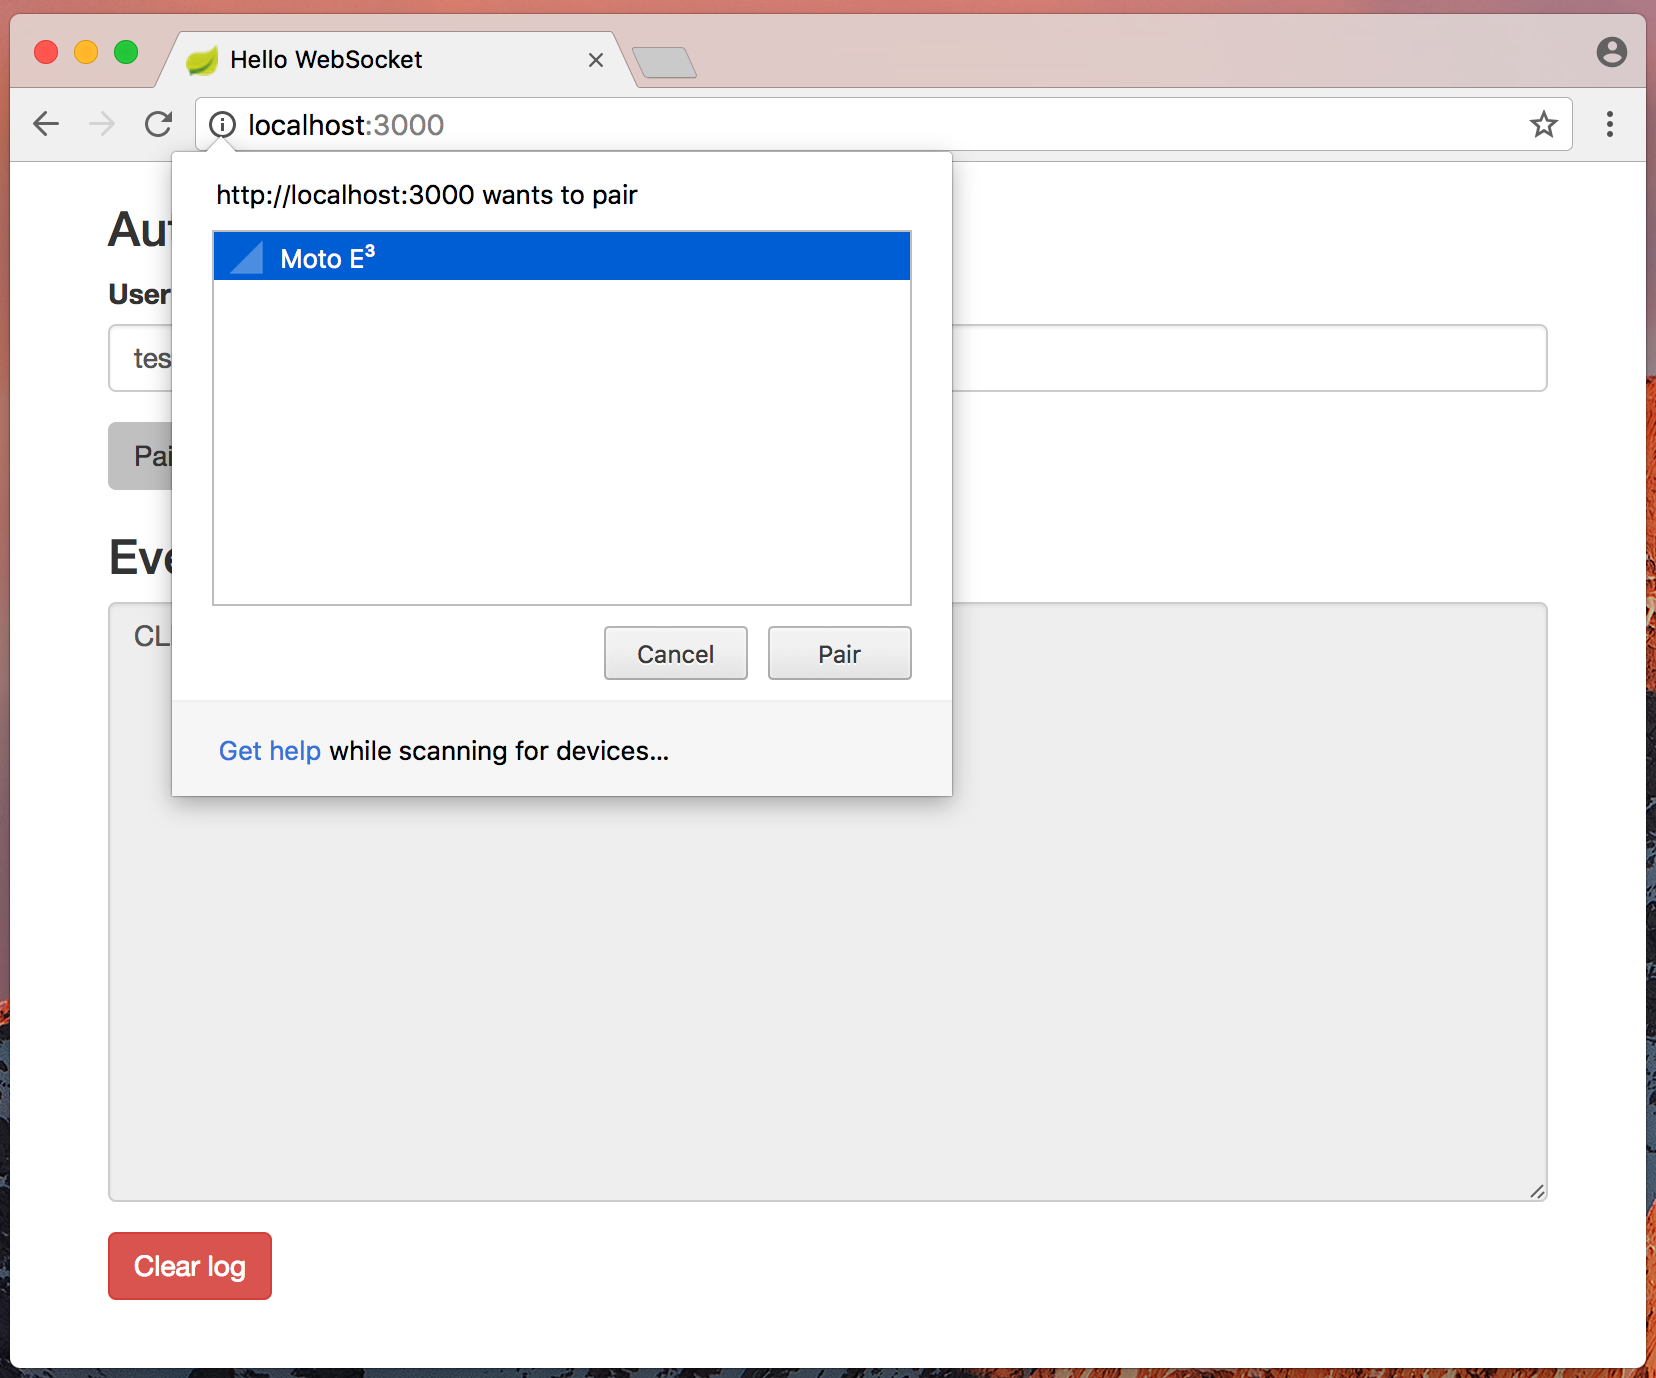
\includegraphics[width=\linewidth]{gfx/paring2} 
       \label{fig:paring}
       \caption{The pairing menu in Chrome}
\end{figure}

\begin{figure}
       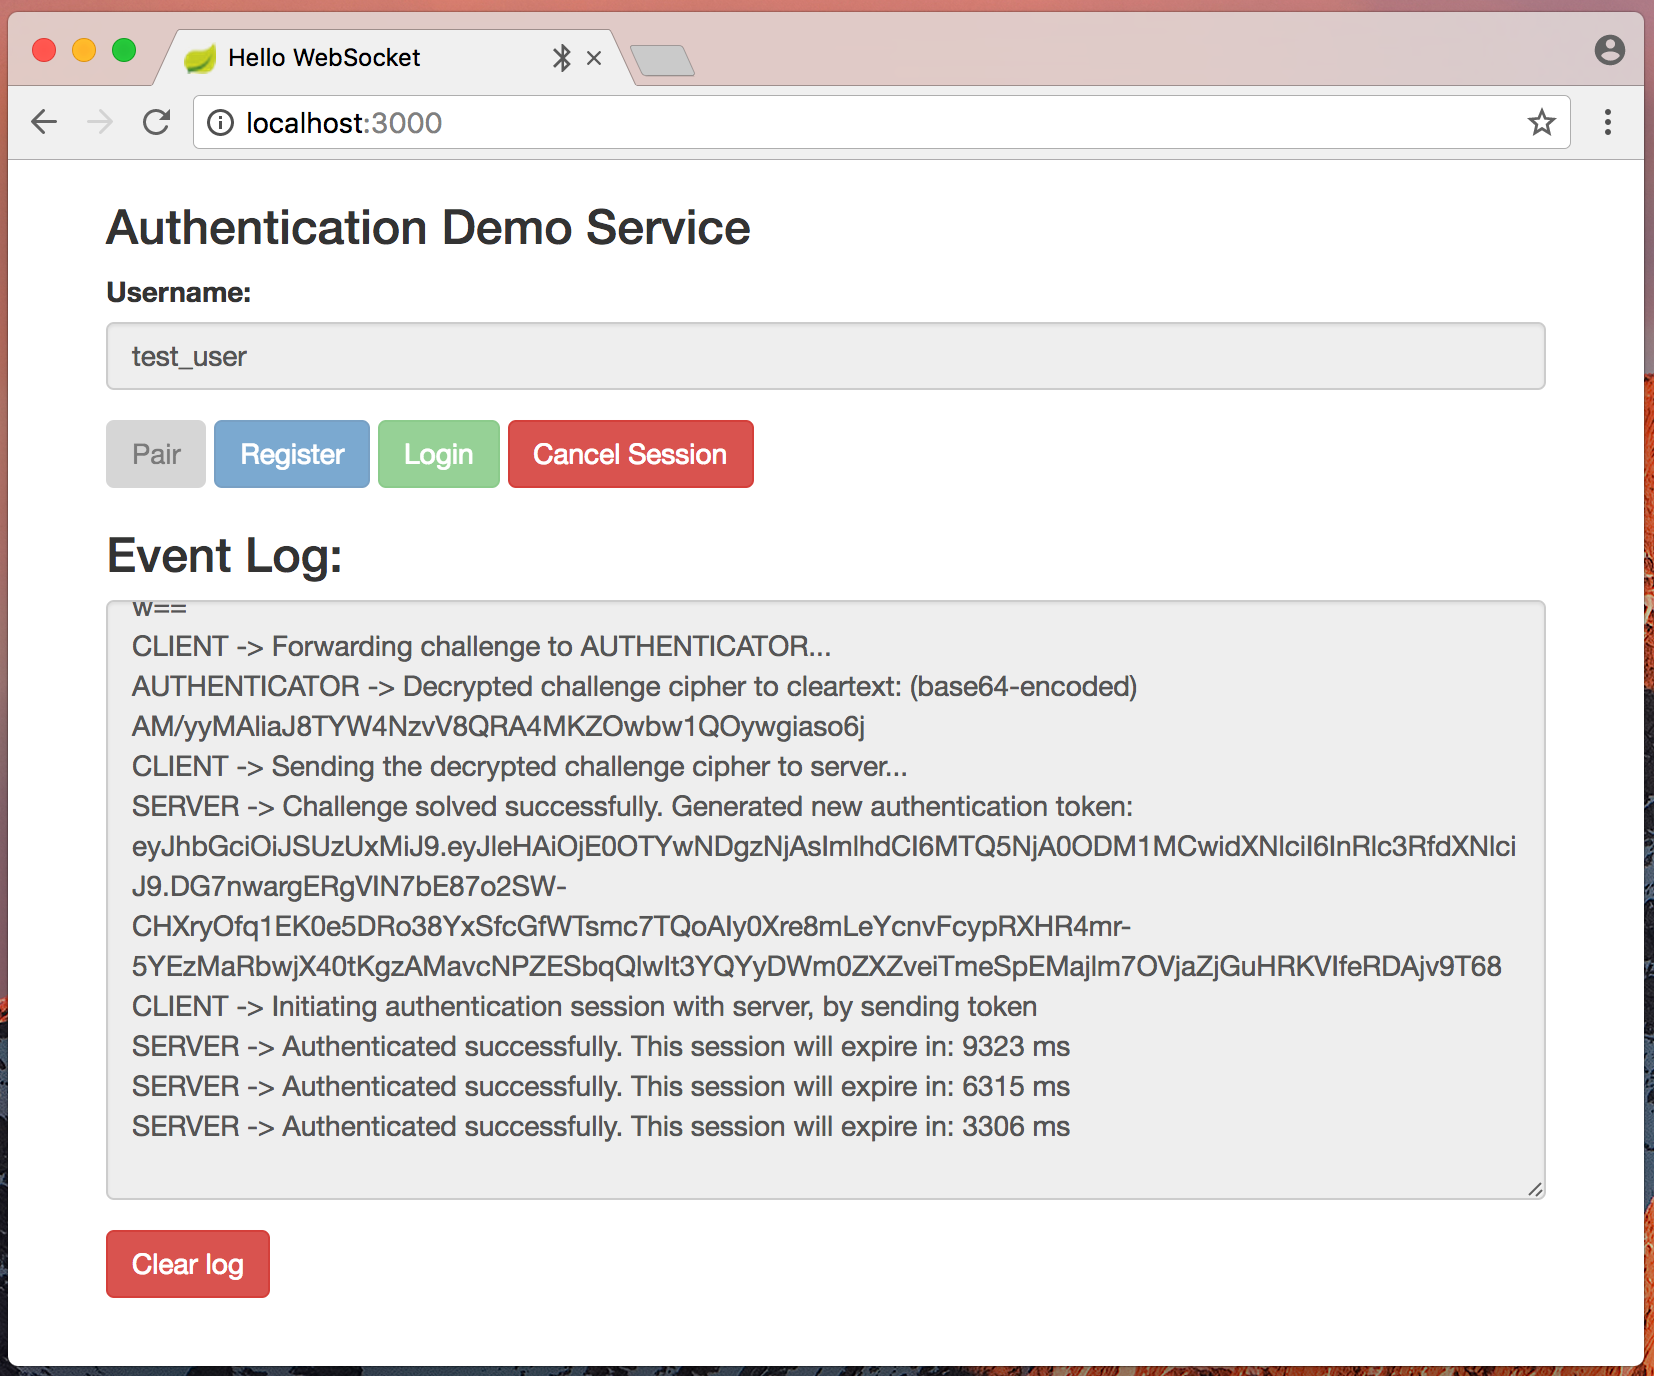
\includegraphics[width=\linewidth]{gfx/login} 
       \label{fig:client}
       \caption{Authenticating with a service in Chrome} 
\end{figure}


\section{Technical Description}
\subsection{Technologies Used}
One clear and important design goal, is to base the prototype implementation of our authentication scheme on commodity hardware and recognized technologies, and as such, this should be clearly reflected in our choice of technologies used. 

The prototype is using the Android platform for the \gls{authenticator} and \gls{sibling}, and developed using Java. All message exchanges between the two devices are handled using the Bluetooth communication protocol. For developing and testing we used Motorolas Moto 360 smartwatch and their $\text{Moto E}^3$ smartphone, although the hardware can be substituted with any two Bluetooth 4.0 LE supported devices that run Android OS and Android Wear OS respectively, with API level 21 or higher. 

The \gls{client} is running a browser application that is served statically as Javascript and HTML files.

We use Bluetooth GATT services to establish a link between \gls{client} and \gls{authenticator}

Generic Attributes (GATT) profile is a feature in Bluetooth LE that allows device discovery based on services without device pairing. A common use of GATT is with sensors, such as heart-rate monitors, that can easily be discovered as used ad-hoc.

We use GATT to expose an authentication service from the \gls{authenticator} that be easily discovered, and can be used without regular device pairing.

Because native GATT service compatibility in the browser is still under active development, the \gls{client} application is only functioning properly in Google Chrome Version 59 or later, which at the time of writing is still in beta release state. When selecting a new unknown device in Chrome for the first time, Chrome as a security requires that the end-user selects the device from a pairing drop-down menu. This is shown in figure~\ref{fig:pairing}. The implementation will, but does not yet support automatically establishing connections to known devices when they come in range.

The \gls{server} is implemented as a server application using Java and the Spring Boot framework. Communication between \gls{client} and server is handled through the WebSocket communication protocol. Public keys user information and generated challenges, are persisted on the server using a MySQL relational database. The server uses the open standard (RFC 7519) JSON Web Tokens (JWT), to issue and verify authentication tokens. The details of token generation and verification are explained in section \ref{sec:tokens} below. 

All cryptographic computations are carried out using the BouncyCastle cryptography Java API. However as the Android platform ships with a limited version of BouncyCastle, and can not be updated to the latest version due to classloader conflicts, we use SpongyCastle to perform cryptographic operations on the \gls{authenticator} and \gls{sibling}. SpongyCastle is essentially the exact same API as BouncyCastle only with a different name, created only with the purpose of enabling the full and updated API of BouncyCastle on the Android platform. The details of our cryptography implementation is explained in section \ref{crypto_impl} below.


\subsection{Algorithms} \label{sec:algorithms}
The implementation of the protocol on the \gls{server}, \gls{authenticator} and \gls{sibling} is based on the algorithms defined below.

\begin{algorithm}
    \BlankLine
    \KwData{Set of public-keys $\{pk_1, pk_2, ..., pk_n \}$}
    \BlankLine
 
    $i \leftarrow recv(C)$
    \tcc*{request from user with id i}
    
    $c = Enc(n,pk_i)$
    \tcc*{generates a random challenge}
    \BlankLine
 
    $send(C,\langle c, i \rangle)$
    \tcc*{sends a challenge to C}
    
    $n' \leftarrow recv(C)$
    \tcc*{receives a response}
    \BlankLine
    
    \If(\tcc*[f]{if the response is valid}){$n = n'$}{
        $send(C, token)$
        \tcc*{then issue a token to C} 
    }
    \BlankLine

 \caption{Service Provider behaviour during authentication}
 \label{alg:servAuth}
\end{algorithm}

\begin{algorithm}
    \BlankLine
    \KwData{Set of key-pairs $\{sk_1, sk_2, ..., sk_n \}$}
    \BlankLine
 
    $\langle c,i \rangle \leftarrow recv(C)$
    \tcc*{receives challenge from C}
    
    $send(As, \langle c, i \rangle)$
    \tcc*{sends challenge to As}
    \BlankLine
    
    $c'_{A} = Dec'(c,sk_{i})$
    \tcc*{partly decrypts}
    
    $c'_{As} \leftarrow recv(As)$
    \tcc*{receives other half from As}
    \BlankLine
    
    $n' = c'_{A} \times c'_{As}$
    \tcc*{combines the parts}
    
    $send(C, n')$ \tcc*{send the token to C}
    \BlankLine
    
 \caption{Authenticator behaviour during authentication}
 \label{alg:authAuth}
\end{algorithm}

\begin{algorithm}
    \BlankLine
    \KwData{Set of private-keys $\{sk_{1}, sk_{2}, ..., sk_{n} \}$}
    \BlankLine
 
    $\langle c,i \rangle \leftarrow recv(A)$
    \tcc*{receives challenge from A}
    
    $c'_{As} = Dec'(c,sk_{i})$
    \tcc*{partly decrypts}
    
    $send(A, c'_{As})$
    \tcc*{sends it to A}
    \BlankLine
    
 \caption{Sibling behaviour during authentication}
 \label{alg:sibAuth}
\end{algorithm}

\clearpage

\subsection{Cryptography Implementation} \label{crypto_impl}
As earlier mentioned, BouncyCastle cryptography API (SpongyCastle on Android) is used, to implement the protocol in practice. 
The different cryptographic operations needed for the \gls{authenticator} and \gls{sibling} are exposed in a shared class which they both use. 
Initially the encryption/decryption scheme to be used, is set to El Gamal without padding, and the bit length is set to 256 for all generated keys (lst. \ref{lst:distEl}, line 47-66). 
 
When a user registers with a new \gls{server}, the \gls{sibling} and the \gls{authenticator} creates an El Gamal key pair each. Key generation is trivial to implement and is handled trough the BouncyCastle API (lst. \ref{lst:distEl}, line 133-152).
To reduce key generation time significantly we avoid generating new large prime numbers required for the El Gamal key parameters $p$ and $g$ each time, but instead uses fixed values for both, that we know are applicable for secure key generation (lst. \ref{lst:distEl}, line 36-37).
When the key pairs are successfully created on each device, the \gls{sibling} sends its public key $y_{as}$ to the \gls{authenticator}, which then adds the \gls{sibling}s public key $y_{as}$ to its own public key $y_a$, resulting in a combined public key $y$ (lst. \ref{lst:distEl}, line 69-85). The \gls{authenticator} now sends its public key $pk$ ($y$ along with parameters $p$ and $g$) to the \gls{server}, where it is stored and associated with the registering user. 

When an authentication request is initiated by the user, the server application encrypts a new challenge cipher, based on the public key it received upon registration. 
The challenge is generated using the formula $(h^2 ~\mathrm{mod}~p)$ where $h$ is an arbitrary integer of $\mathbb{Z}^*_p$ in the range $\big\{ 2, ..., p-2 \big\}$. Naturally, the server also uses the El Gamal No Padding cipher to perform encryption. The server stores the challenge in the database in both cleartext and ciphertext along with an expiration timestamp indicating how long the \gls{server} accepts responses for the generated challenge (lst. \ref{lst:chalService}, line 46-81). 

The challenge is sent to the \gls{authenticator}, which will now decrypt the cipher in cooperation with its \gls{sibling}. As shown in algorithm: \ref{alg:authAuth}, the \gls{authenticator} sends a copy of the challenge to the \gls{sibling} immediately upon receiving it from the server. Hereafter both devices will perform a partial decryption of the cipher, using their individual private key. This is done by first splitting the challenge cipher into two parts: $\alpha$ and $\beta$ (lst. \ref{lst:chalService}, line 168-181). Partial decryption is then done by: $\left[\beta^{(p-1-x)} ~\mathrm{mod}~p\right]$, where $x$ is the private key, and $p$ is the common security parameter of the public key (lst. \ref{lst:chalService}, line 98-109). Note that, as $p-1$ is the order of the group used, then $h^{(p-1)} = 1$ with $h \in \mathbb{G}$.
\begin{align*}
    && c'_i = \beta^{(p-1-x_i)} = \frac{\beta^{(p-1)}}{\beta^{x_i}} = \beta^{-x_i}
\end{align*}

Note that this is different from the partial decryption as defined in the protocol section. This is due to the fact that division in groups in Bouncy Castle is defined as $a / b \stackrel{def}{=} \left[ ab^{-1}~\mathrm{mod}~p \right]$.

The main difference between the algorithm  executed by the \gls{authenticator} (algorithm~\ref{alg:authAuth}) and the one (algorithm~\ref{alg:sibAuth}) executed by the \gls{sibling}, is that the \gls{sibling} sends the result of its decryption directly to the \gls{authenticator}, which combines the two partial ciphers into the correct cleartext solution of the challenge. The \gls{authenticator} does so by computing $\left[\alpha \cdot c'_1 \cdot c'_2 ~\mathrm{mod}~p\right]$ where $c'_1$ and $c'_2$ are the partial ciphers from the \gls{authenticator} and \gls{sibling} (lst. \ref{lst:chalService}, line 87-96). This formula computes the solution to the challenge, which is then sent back to the server, so it can complete the last step of its algorithm (algorithm~\ref{alg:servAuth}), which is to authenticate the \gls{client}.


\subsection{Token Issuing and Verification} \label{sec:tokens}
The prototype is using JSON Web Tokens (jwt.io), to issue new authentication tokens on the server, upon receiving a correct solution to a challenge. The tokens are signed digitally with a public/private key pair using RSA. JWT tokens can carry different kinds of information with them, such as a timestamp to indicate an expiration time for the token. 
Our implementation uses the JWT Java API provided by Auth$0$(\href{https://github.com/auth0/java-jwt}{GitHub page}). The server generates a new RSA key pair upon server start (lst. \ref{lst:tokenService}, line 37-52). When a new token has to be issued for a given user, the following information is stored in the token: a timestamp for when the token was issued, a timestamp for when the token is set to expire, the username of the authenticated user. The token is then signed with RSA512 using the private key that was generated on server start (lst. \ref{lst:tokenService}, line 54-73). Verification is done using the RSA public key. The verification function of the API takes an RSA public key as input, and checks and that the token is signed by the corresponding private key and not expired yet (lst. \ref{lst:tokenService}, line 75-93). 


\section{Prototype Evaluation}\label{sec:prot_eval}
We evaluate our implementation based on the framework proposed by \citet{bonneau2012quest}, in a similar manner to how we evaluated the design of our scheme in section \ref{sec:rating_process}, and other schemes in chapter \ref{ch:review}. 

\begin{table}[bth]
\centering
\begin{wide}
\resizebox{\linewidth}{!}{
%\rotatebox{270}{
\setlength\tabcolsep{1.8pt}
\begin{tabular}{r|c|cccccccccc|cccccc|ccccccccccccc}

\multicolumn{2}{c}{} &
\multicolumn{10}{c}{\textbf{Usability}} &
\multicolumn{6}{c}{\textbf{Deployability}} &
\multicolumn{13}{c}{\textbf{Security}}\\
\multicolumn{31}{c}{}
\\

& \rot{\textit{Reference}} &
\rot{\textit{Memorywise-Effortless}} &
\rot{\textit{Scalable-for-Users}} &
\rot{\textit{Nothing-to-Carry}} &
\rot{\textit{Physically-Effortless}} &
\rot{\textit{Easy-to-Learn}} &
\rot{\textit{Efficient-to-Use}} &
\rot{\textit{Infrequent-Errors}} &
\rot{\textit{Easy-Recovery-from-Loss}} &
\rot{\textit{Awareness}} &
% \rot{\textit{Multi-User-Support}} &
\rot{\textit{No-Config}} &
\rot{\textit{Accessible}} &
\rot{\textit{Negligible-Cost-per-User}} &
\rot{\textit{Server-Compatible}} &
\rot{\textit{Browser-Compatible}} &
\rot{\textit{Mature}} &
\rot{\textit{Non-Proprietary}} &
\rot{\textit{Resilient-to-Physical-Observation}} &
\rot{\textit{Resilient-to-Targeted-Impersonation}} &
\rot{\textit{Resilient-to-Throttled-Guessing}} &
\rot{\textit{Resilient-to-Unthrottled-Guessing}} &
\rot{\textit{Resilient-to-Internal-Observation}} &
\rot{\textit{Resilient-to-Leaks-from-Other-Verifiers}} &
\rot{\textit{Resilient-to-Phishing}} &
\rot{\textit{Resilient-to-Theft}} &
\rot{\textit{No-Trusted-Third-Party}} &
\rot{\textit{Requiring-Explicit-Consent}} &
\rot{\textit{Unlinkable}} &
\rot{\textit{No-Intermediary-Knowledge}} &
\rot{\textit{Continuous}} \\ \hline

Scheme design & &
\CIRCLE     & %Memorywise-Effortless
\CIRCLE     & %Scalable-for-Users
\Circle     & %Nothing-to-Carry
\CIRCLE     & %Physically-Effortless
\CIRCLE     & %Easy-to-Learn
\CIRCLE     & %Efficient-to-Use
\CIRCLE     & %Infrequent-Errors
            & %Easy-Recovery-from-Loss
\CIRCLE     & %Awareness
%           & %Multi-User-Support
            & %No-Pairing
\CIRCLE     & %Accessible
\Circle     & %Neglible-Cost-per-User
            & %Server-Compatible
            & %Browser-Compatible
            & %Mature
\CIRCLE     & %Non-Proprietary
\CIRCLE     & %Resilient-to-Physical-Observation
\CIRCLE     & %Resilient-to-Targeted-Impersonation
\CIRCLE     & %Resilient-to-Throttled-Guessing
\CIRCLE     & %Resilient-to-Unthrottled-Guessing
\Circle     & %Resilient-to-Internal-Observation
\CIRCLE     & %Resilient-to-Leaks-from-Other-Verifiers
\CIRCLE     & %Resilient-to-Phishing
\Circle     & %Resilient-to-Theft
\CIRCLE     & %No-Trusted-Third-Party
\Circle     & %Requiring-Explicit-Consent
\CIRCLE     & %Unlinkable
\CIRCLE     & %No-Intermediary-Knowledge
\CIRCLE       %Continuous
\\ \hline

Prototype Implementation & \cite{stajano2011pico} &
\CIRCLE     & %Memorywise-Effortless
\CIRCLE     & %Scalable-for-Users
\Circle     & %Nothing-to-Carry
\CIRCLE     & %Physically-Effortless
\CIRCLE     & %Easy-to-Learn
\Circle     & %Efficient-to-Use
\CIRCLE     & %Infrequent-Errors
            & %Easy-Recovery-from-Loss
\CIRCLE     & %Awareness
%           & %Multi-User-Support
\CIRCLE     & %No-Pairing
\CIRCLE     & %Accessible
\Circle     & %Neglible-Cost-per-User
\Circle     & %Server-Compatible
\Circle     & %Browser-Compatible
            & %Mature
\CIRCLE     & %Non-Proprietary
\CIRCLE     & %Resilient-to-Physical-Observation
\CIRCLE     & %Resilient-to-Targeted-Impersonation
\CIRCLE     & %Resilient-to-Throttled-Guessing
\CIRCLE     & %Resilient-to-Unthrottled-Guessing
\Circle     & %Resilient-to-Internal-Observation
\CIRCLE     & %Resilient-to-Leaks-from-Other-Verifiers
\CIRCLE     & %Resilient-to-Phishing
\Circle     & %Resilient-to-Theft
\CIRCLE     & %No-Trusted-Third-Party
\Circle     & %Requiring-Explicit-Consent
\CIRCLE     & %Unlinkable
\CIRCLE     & %No-Intermediary-Knowledge
\CIRCLE       %Continuous
\\ \hline
\multicolumn{31}{r}{

\CIRCLE~=~offers the benefit 
\quad \Circle~=~almost offers the benefit
%\quad \textit{no circle}~=~does not offer the benefit 
\quad ?~=~not known}
\quad \\

\end{tabular}}
\end{wide}

\caption[Overview of benefits of our prototype]{Comparing the (envisioned) benefits of our design with the actual benefits of our implementation.}
\label{table:property_table2}
\end{table}

\subsection{Rating process}
To avoid repeating ourselves, we only describe the rating rationale behind the specific benefits of the prototype implementation that differ from the scheme design. 
We grant the prototype \textit{No-Config} as it actually offers this benefit according to our definition, since there is no difference between the required effort from the user, the first time or sub sequential times it is used on any client. This may appear more beneficial than it actually is. In reality, a pairing step between \gls{authenticator} and \gls{client}, becomes something the user has to do every single time he starts a new authentication or registration request, instead of something that should only be done once on each \gls{client}, which obviously is less desirable. This is also the reason why we only grant the prototype \textit{Quasi-Efficient-to-Use} as the user is required to select the correct \gls{authenticator} from a list of devices, on the \gls{client}, every time the browser reloads the page. 
While deployability benefits are not prioritized in the scheme design, it was discovered during implementation that it was actually possible to achieve both \textit{Browser-} and \textit{Server-Compatibility} to some extent. We award the prototype \textit{Quasi-Browser-Compatibility} as no browser plugins or additional software is required to run on the \gls{client} machine, in order to use the prototype. However the browser support for Bluetooth GATT services is used in the implementation, is still in a beta state, and currently only works in a limited amount of browsers. Assuming that Bluetooth communication directly through the browser, becomes more common and widely supported in the future, we award \textit{Quasi-Browser-Compatibility}.
We award \textit{Quasi-Server-Compatibility}, since servers that already use JWT tokens for authentication, can become compatible with the scheme, without a complete re-implementation of its authentication infrastructure . 
Essentially such servers do not require changes, in terms of how it is determined whether a user is authorized to access a requested resource or not. Instead, a change is needed, in the way it is determined whether a user is entitled to receive an authentication token or not, which today is typically done by verifying a user's username/password credentials. 